Alicia y Benito usan un programa para llevar la cuenta
del marcador de sus partidos de tenis de mesa.
Cada vez que alguno de ellos gana un punto,
hace clic en el botón con su nombre,
y el marcador es actualizado.

Un partido de tenis de mesa está dividido en 7 juegos.
Cuando alguien gana 11 puntos,
el juego se termina y comienza el juego siguiente.

\begin{tikzpicture}[scale=5.5]
  \node (A) at (0, 0) {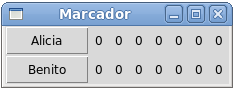
\includegraphics[scale=0.55]{marcador/marcador-0.png}};
  \node (B) at (1, 0) {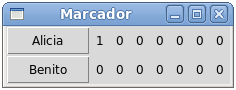
\includegraphics[scale=0.55]{marcador/marcador-1.png}};
  \node (C) at (2, 0) {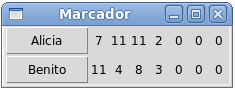
\includegraphics[scale=0.55]{marcador/marcador-2.png}};
  \draw[-latex'] (A) -- (B);
  \draw[-latex'] (B) -- (C);
  \node[font=\footnotesize, anchor=baseline, node distance=6ex, below of=A] {Marcador inicial};
  \node[font=\footnotesize, anchor=baseline, node distance=6ex, below of=B] {Después de hacer clic en Alicia};
  \node[font=\footnotesize, anchor=baseline, node distance=6ex, below of=C] {Después de muchos clics};
\end{tikzpicture}

El programa define dos listas de modelos,
llamadas \li!modelos_a! y \li!modelos_b!,
que guardan los puntos ganados en cada juego
por el jugador respectivo.
Por ejemplo, \li!modelos_a[3]! guarda los puntos
que ha ganado Alicia en el cuarto juego
(recuerde que se cuenta desde cero).

Además,
hay un modelo que guarda cuál es el juego actual
(un número entre 0 y 6):
\lstinputlisting[linerange=JUEGO\ ACTUAL-FIN\ JUEGO\ ACTUAL]{marcador/pauta-marcador.py}

Los botones fueron creados de la siguiente manera:
\lstinputlisting[linerange=BOTONES-FIN\ BOTONES]{marcador/pauta-marcador.py}

Escriba el código del controlador \li!punto_a!.

